\chapter{Migration de code}
\label{ch:task_migration}

Ce chapitre traite du mécanisme de diffusion de modules qui est utilisé dans
la migration de code. Notre approche exploite la sérialisation des objets
Scheme, le langage Termite et l'installation automatique des modules durant
l'exécution.

La migration de code entre les nœuds d'un système distribué n'est possible
que si chaque nœud utilise la même version de Gambit configuré avec les
mêmes paramètres. Des versions différentes de Gambit vont compiler le code
différemment, ce qui peut rendre la sérialisation/désérialisation possiblement
incompatible. La compilation des modules doit utiliser les mêmes déclarations
et optimisations Scheme. Le compilateur C, le système d'exploitation, la taille
des mots mémoires n'ont pas d'importance.

\section{Systèmes distribués}

Les systèmes distribués sont constitués d'un ensemble de nœuds interconnectés
de calculs. Les nœuds interagissent par l'envoi et la réception de message au
sein d'un réseau de communication. Chaque nœud a un but spécifique. Le
\textit{Web} est un exemple notable représentatif.  Il est composé de clients
et de serveurs qui exécutent des applications clients et serveurs différentes.

L'implémentation d'un système distribué inclut le développement des
applications installées sur les nœuds et la logique d'interaction entre les
nœuds. Il est possible de voir l'ensemble des programmes sur les nœuds comme un
programme global. Les problèmes discutés dans ce chapitre sont les suivants:

\begin{itemize}

  \item {\bf RPC:} Comment l'appel distant à une procédure (RPC)
    implémentée quand l'envoyeur et le receveur ne sont pas conçus
    ensemble?

  \item {\bf Mise à jour de code:} Comment la mise à jour du programme d'un
    nœud est effectuée lors d'un \textit{bugfix} ou lorsqu'une nouvelle
    version est disponible?

  \item {\bf Migration de tâche:} Comment déplacer un service sur un nouveau
    nœud quand le système sous-jacent est sur un système d'exploitation
    différent, à une architecture différente, etc.?

  \item {\bf Opération continue:} Comment éviter les interruptions dans les
    situations précédentes?

\end{itemize}

Le langage Termite Scheme~\cite{DBLP:conf/erlang/Germain06} a été conçu
pour simplifier l'implémentation de systèmes distribués et fournit
certaines solutions aux problèmes de ces systèmes. Le langage Termite Scheme est
fortement inspiré des concepts du langage de programmation d'Erlang avec la
syntaxe et la sémantique de Scheme. Une fonctionnalité intéressante qui est
absente en Erlang est la capacité d'envoyer une continuation en message.
Termite Scheme est implémenté sur le système Gambit Scheme qui offre
une façon de sérialiser la plupart des objets Scheme incluant les
procédures et les continuations.

La sérialisation de procédures est un outil utile pour implémenter
un protocole RPC. En plus des procédures, il est possible de sérialiser
des continuations. Une continuation est une structure de donnée qui capture
l'état d'un processus. Donc il est possible de transmettre l'état d'un
processus sur un autre nœud.

L'implémentation originale de Termite avait certaines limitations
lors de la sérialisation des procédures et des continuations. Dans
le cas interprété, les procédures et les continuations sont transmises
sans problème entre les nœuds. Dans le cas compilé, il faut que
chaque nœud possède le code compilé des procédures qui sont transmises.


\section{Communication dans Termite}

L'ensemble des données transmises sont sérialisées par la procédure
\lstcode{object->u8vector} qui prend en paramètre l'objet à sérialiser et
optionnellement une procédure \textit{transform} qui est appellé sur tous les
sous-objets dans l'objet pour personnaliser le processus de sérialisation. Le
résultat est un \texttt{u8vector} (vector d'octets).

La sérialisation de la plupart des objets utilise les bits de poids fort du
premier octet pour indiquer le type de l'objet. Les autres des bits du premier
octet sont utilisés pour encoder des propriétés de base comme la longueur de
l'objet (si la valeur peut être encodé avec ces bits).

La sérialization du vecteur \texttt{\#(1 2 3)} est représenté par les 4 octets
\texttt{\#x23} \texttt{\#x51} \texttt{\#x52} \texttt{\#x53}.  Le premier octet
indique que c'est un type vector de longueur 3, les autres octets représentent
les nombre 1, 2 et 3.  La sérialisation d'une procédure contient le nom de
celle-ci et un entier qui l'identifie. La figure~\ref{fig:proc_serialization}
montre un exemple de la sérialisation d'une procédure compilée. Cette
représentation est conçue pour être compacte et éviter la redondance dans les
données. En plus, elle est indépendante de l'architecture de la machine.

\begin{figure}[ht]
  \centering
  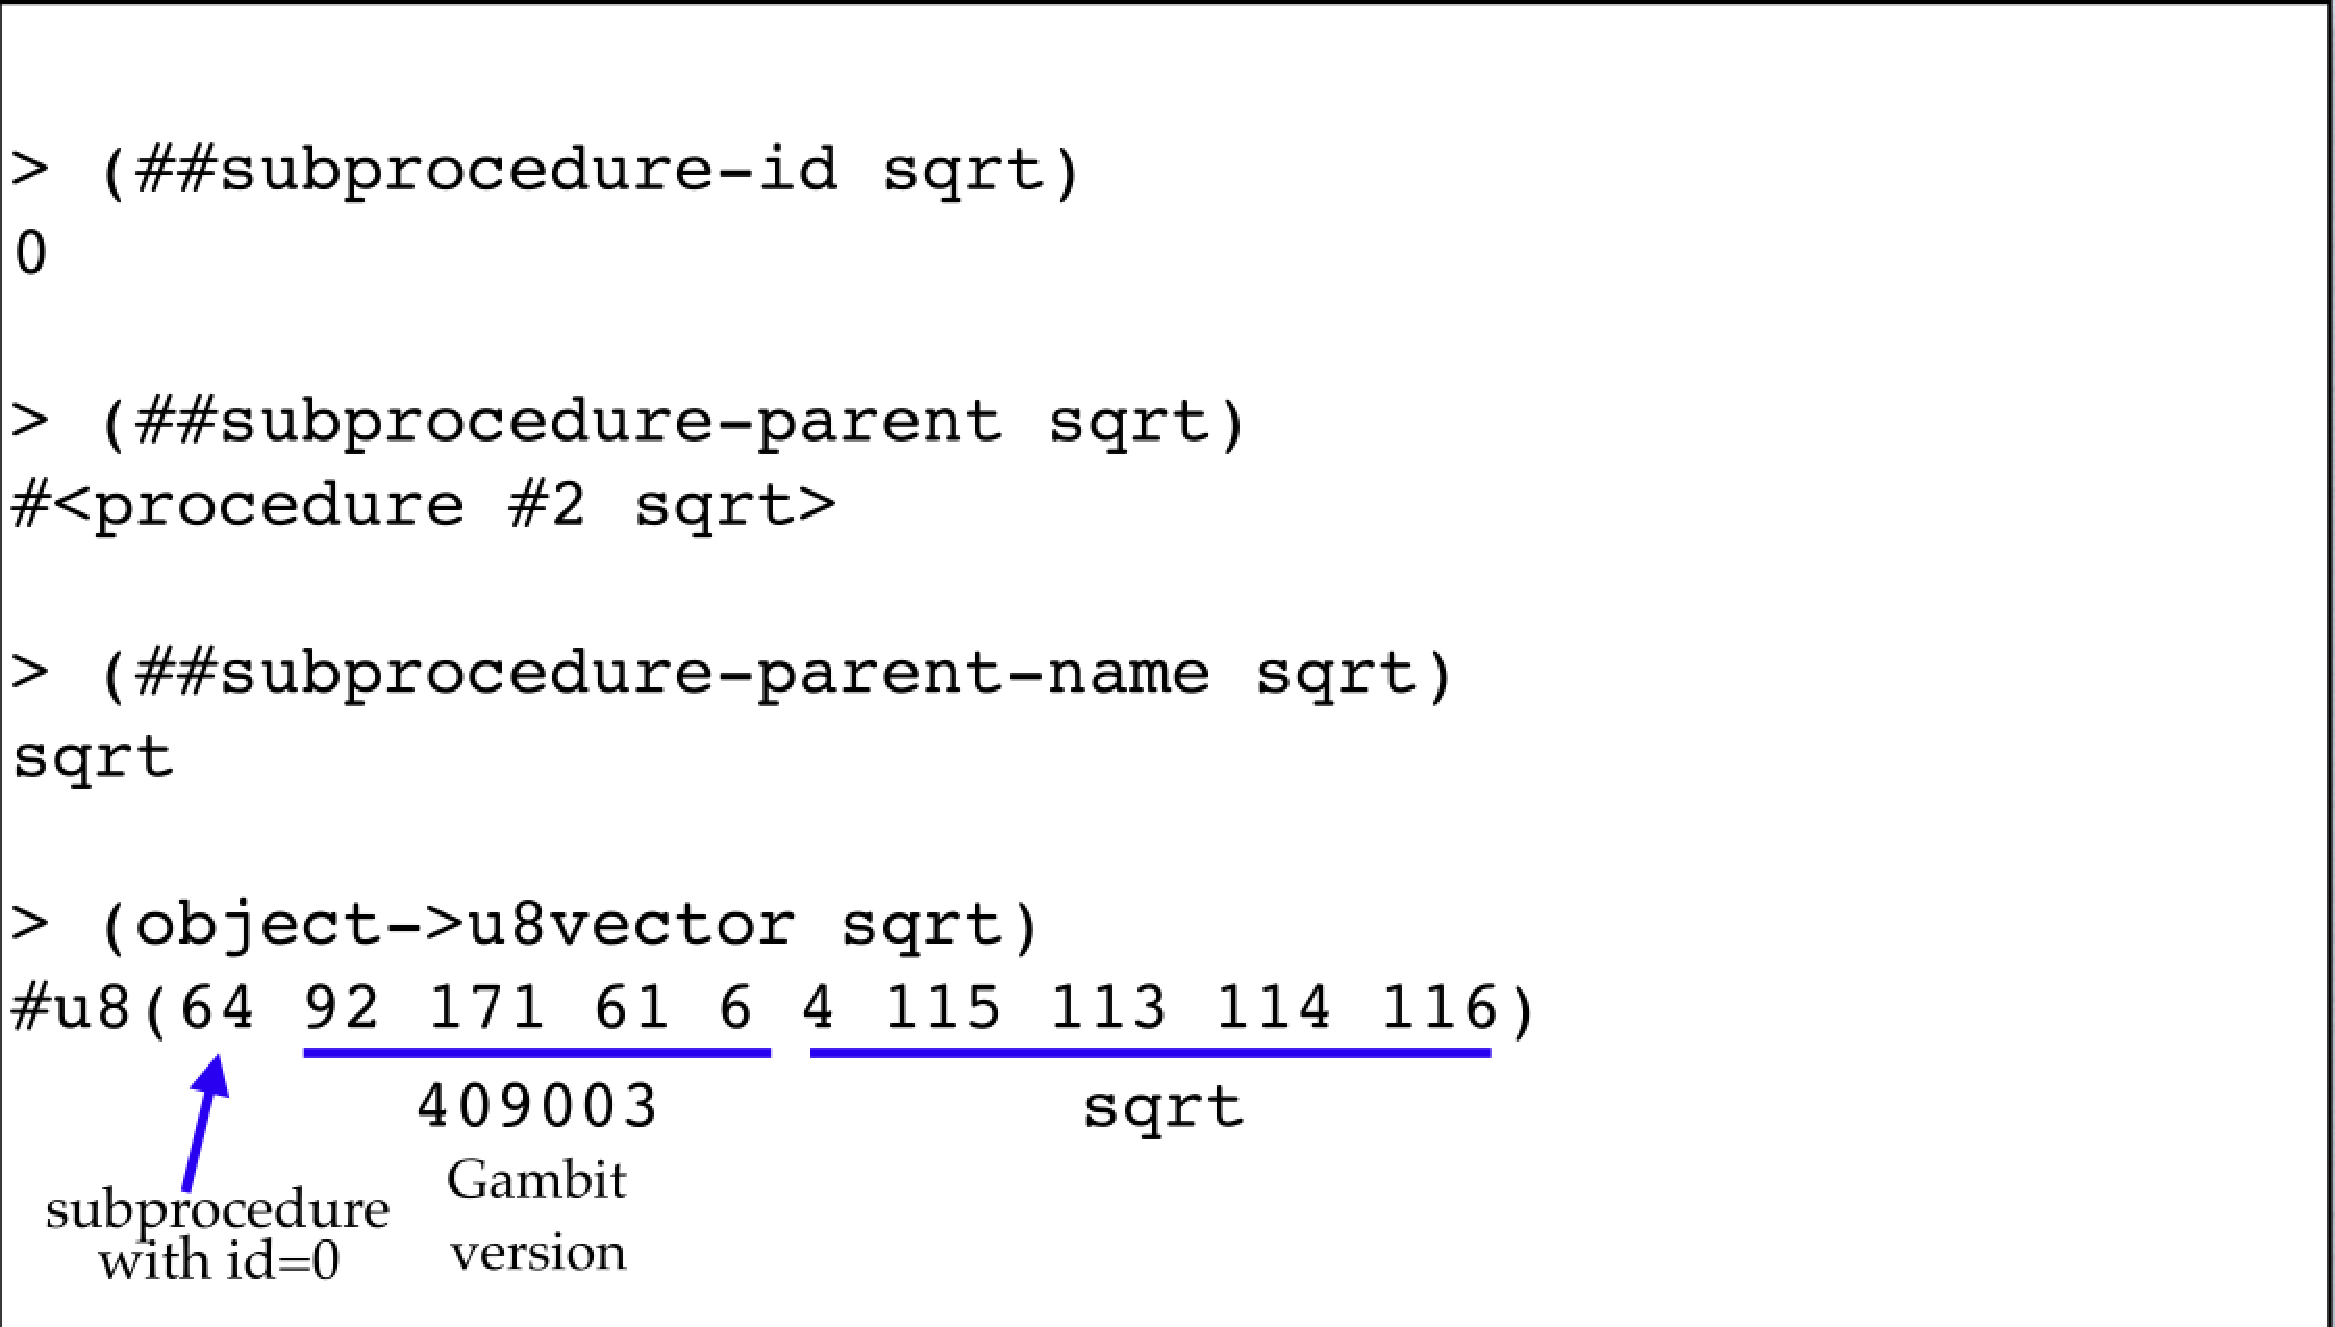
\includegraphics[scale=0.25]{figures/proc-serialization}
  \caption{La représentation du résultat de la sérialisation en \texttt{u8vector} de la procédure
    \texttt{sqrt}.}
  \label{fig:proc_serialization}
\end{figure}

\section{\textit{Hook} des procédures inconnues}
%
Le système Termite permet la migration de code compilé avec les procédures
\lstcode{object->u8vector} et \lstcode{u8vector->object}. Ces procédures
effectuent respectivement la sérialisation et la désérialisation.
La sérialisation d'une procédure est encodée par le nom de la procédure et
un entier qui l'identifie (\texttt{id}).

Le nom qualifié de la procédure (i.e. qui contient un \texttt{\#}) est composé
de l'espace de nom et du nom court. La procédure \lstcode{_hamt#make-hamt} est
dans l'espace de nom \lstcode{_hamt} et à un nom court \lstcode{make-hamt}.
L'espace de nom dans un module qui est hébergé correspond au \lstcode{module-ref}
qui est dans le cas des modules hébergés l'URL du dépôt contenant
le code du module.

Dans le processus de désérialisation, le nom de la procédure et le \texttt{id}
sont utilisés pour retrouver la procédure. Un \textit{hook} est invoqué
si la procédure n'existe pas dans le processus courant. Le but de
ce \textit{hook} est de dynamiquement installer et charger le module 
qui implémente la procédure inconnue.

%\newpage
\section{Exemple de migration de code}

Pour montrer les capacités du système nous avons conçu un scénario de mise à
jour de code entre deux nœuds. Un nœud qui exécute l'application compilée et un
nœud qui exécute le code qui effectue la mise à jour de l'application sans
interrompre le service.

Les deux nœuds ont la même version de Gambit, car la mise à jour de code
compilé requiert une version uniforme de Gambit. La représentation des
\textit{subprocedure} peut être inconsistante entre les versions de Gambit.

L'application est une horloge programmable écrite en Termite Scheme qui affiche
l'heure dans un certain fuseau horaire configurable. Cette application a un bogue
d'affichage volontaire qui se produit lorsque l'horloge passe de {\tt 12h59} à
{\tt 1h00}. L'affichage montre {\tt 1h009} au lieu de {\tt 1h00}.

Cette horloge offre un API simple:
\begin{itemize}
  \item La modification du fuseau horaire est faite en envoyant
    un message (nombre entier).

  \item Le message \lstcode{timezone-get} permet de récupérer
    le fuseau horaire courant.

  \item Le message \lstcode{update-code} permet la mise à jour
    dynamique du code du serveur.

  \item Tous les autres messages sont rejetés par le serveur.
\end{itemize}

L'horloge programmable est démarrée sur le nœud, par exemple un raspberry pi 4.
L'heure affichée n'est pas dans le bon fuseau horaire, donc nous utilisons
le programme \texttt{timezone-set.scm} de la figure~\ref{fig:termite_clock_client}
pour configurer le bon fuseau horaire. Par exemple, pour assigner le fuseau 4
nous invoquons le programme comme suit: \lstcode{gsi timezone-set.scm 4}.

L'horloge est maintenant dans le fuseau horaire 4. Une nouvelle version de
l'horloge programmable est disponible. Le service ne doit pas être interrompu.
Par commodité l'horloge supporte un message qui permet la mise à jour
du code qui est (\lstcode{update-code}).

Le programme \texttt{updater.scm} de la figure \ref{fig:termite_clock_client}
permet d'envoyer la nouvelle version de l'horloge programmable. La mise à jour
est faite en envoyant une procédure ou une continuation qui contient la logique
(comme dans la figure~\ref{fig:buggy_pong_server}). Dans ce cas, c'est une
procédure qui est envoyée pour mettre à jour le horloge programmable.

La procédure envoyée provient du module
\texttt{github.com/frederichamel/termite-clock@v2} qui est la nouvelle version
de l'horloge. L'espace de nom de ce module est
\texttt{github.com/frederichamel/termite-clock@v2\#}. Le nom de la procédure
est \texttt{clock-thread-loop} dans l'espace de nom de ce module.

La sérialisation de la procédure contient le nom de la procédure incluant
l'espace de nom. Le nœud Termite qui roule l'application de l'horloge
programmable a configuré l'installation automatique des modules. Même si la
procédure n'existe pas sur le nœud Termite de l'horloge programmable le système
va l'installer, le compiler et le charger dynamiquement.\\

% Le code exécuté par la boucle principale est présent dans la figure
% \ref{fig:termite-clock@v1}. L'affichage de l'heure est actualisé à une
% fréquence constante.

\begin{figure}[ht]
  \centering\fontsize{12}{8}
  \lstset{language={Scheme},frame=single}
\begin{mplisting}{1}
;; clock-app.scm
(import (termite))
(import (github.com/frederichamel/termite-clock @v1))

;; Should be integrated in the system.
(##unknown-procedure-handler-set!
  (lambda (name id)
    (let* ((name-str (##symbol->string name))
           (proc/ns (##reverse-string-split-at name-str #\#)))
      (and (##pair? (##cdr proc/ns))
           (let ((mod-name (##last proc/ns)))
             (##load-module (##string->symbol mod-name))
             (let ((proc (##get-subprocedure-from-name-and-id name id)))
               proc))))))

(define node (make-node "b.local" 3000))

(define (start)
  (node-init node)
  (display "\033[H\033[J") ;; clear screen
  (clock-start 'clock-app)
  (wait-for (resolve-service 'clock-app)))

(start)
\end{mplisting}
  \caption{Le code du serveur qui configure le \textit{hook}
    qui résout les références à des procédures inconnues.
    C'est effectué avec la procédure
    \lstcode{\#\#unknown-procedure-handler-set!}.}
  \vspace*{4ex}
\end{figure}


\begin{figure}[ht]
  \centering\fontsize{12}{8}
  \lstset{language={Scheme},frame=single}
\begin{mplisting}{1}
(define (clock-thread-loop timezone)
  (let tick ()
    (let* ((now (time->seconds (current-time)))
           (next (* 0.5 (floor (+ 1 (* 2 now))))) ;; next 1/2 second
           (timeout (seconds->time next)))
      (let wait ()
        (recv
          ((from tag timezone) (where (integer? timezone))
           (! from (list tag 'ok)) ;; send confirmation
           (clock-thread-loop timezone))

          ((from tag ('update-code k))
           (! from (list tag 'ok)) ;; send confirmation
           (k timezone))

          ((from tag 'timezone-get)
           (! from (list tag timezone))
           (wait))

          (after timeout
           (clock-update next timezone)
           (tick)))))))
\end{mplisting}
  \caption{Extrait du code de l'horloge programmable.}
  \label{fig:termite-clock@v1}
  \vspace*{4ex}
\end{figure}

\begin{figure}[ht]
  \centering\fontsize{12}{8}
  \lstset{language={Scheme},frame=single}
  \begin{tabular}{c}
\begin{mplisting}{1}
;; config.scm
(define local    (make-node "a.local" 3000)) ;; x86 arch
(define remote   (make-node "b.local" 3000)) ;; ARM arch
\end{mplisting}\\[5ex]
\begin{mplisting}{1}
;; timezone-set.scm
(import (termite))

;; Configure the current node.
(include "config.scm")

;;; Update timezone
(node-init local)
(let* ((args (command-line))
       (rest (cdr args)))
  (if (or (null? rest)
          (pair? (cdr rest)))
      (!? (remote-service 'clock-app remote) 0) ;; => 'ok
      (let ((timezone (string->number (car rest))))
        (!? (remote-service 'clock-app remote) (or timezone 0))))) ;; => 'ok
\end{mplisting}\\[5ex]
\begin{mplisting}{1}
;; updater.scm
(import (termite))
(import (github.com/frederichamel/termite-clock @v2))

;; Configure the current node.
(include "config.scm")

(node-init local)
(!? (remote-service 'clock-app remote)
    (list 'update-code clock-thread-loop)) ;; => 'ok
\end{mplisting}
  \end{tabular}
  \caption{Les applications clients qui interragissent avec
    l'horloge programmable. Il y a le programme qui modifie
    le timezone de l'horloge programme dans \texttt{timezone-set.scm}.
    Il y a le programme de mise à jour de l'horloge programmable
    dans \texttt{updater.scm}.}
  \vspace*{4ex}
  \label{fig:termite_clock_client}
\end{figure}

\section{Conclusion}
Ce chapitre présente le mécanisme de diffusion des modules utilisés
dans la migration de code. L'exemple de l'horloge montre une application
de mise à jour dynamique du code qui est possible grâce au mécanisme
de diffusion du code. Notre implémentation de ce système permet l'installation
de la nouvelle version d'un module qui répare un bug dans l'application
\texttt{termite-clock} dans arrêter l'application.

Ce mécanisme est utile pour mettre à jour un serveur évolutif sans
l'interrompre. Notre approche permet la diffusion de modules entre les nœuds
d'un système distribué. Nous évaluons les performances de notre
système dans le prochain chapitre.
